\section{Genetic Algorithms}

\subsection{History}\todo{Decide whether to keep this section}

Genetic algorithms (GAs) are a type of meta-heuristic optimisation technique that employ the same rationale as classical evolution seen in nature.

Genetic Algorithms can trace their origins back to the late 1960s when they were first proposed by John Holland, though he then referred to them as \textit{Genetic Plans}\footnote{This distinction was made to emphasise the \textit{``centrality of computation in defining and implementing the plans''}~\cite{hollandAdaptationNaturalArtificial1992}}. Holland went on to write the first book on the subject titled \textit{Adaptation in Natural and Artificial Systems}\cite{hollandAdaptationNaturalArtificial1992} in 1975. The field did not find much reception with Holland stating in the preface to the 1992 rerun:

\begin{displayquote}
\textit{``When this book was originally published I was very optimistic, envisioning extensive reviews and a kind of `best seller' in the realm of monographs. Alas! That did not happen.''}
\end{displayquote}

However, in the early nineties, Genetic algorithms surged in popularity along with the area of Artificially Intelligent planning as a whole, leading to Holland republishing his book and solidifying his position as the field's founder.

\subsection{Definition}
In a general sense, optimisation techniques work to find the set of parameters $\mathcal{P}$ that minimise an objective function $\mathcal{F}$. 
Genetic algorithms approach this by representing these sets as individuals in a population, $P$. Over the course of multiple generations, the best solutions are determined and promoted until termination criteria are met or the maximum number of generations is reached.

As our candidates are essentially a collection of parameters to the function we are trying to optimise, we can extend our metaphor further by mapping each element of a individual to a \textit{gene} in a individual's genome. 

The representation we use in a GA is problem-specific. Often we have to provide functions to facilitate the mapping between the problem-specific set of possible solutions and the encoded genotype space in which we optimise. The most basic representation being a string of binary numbers.

An individual's characteristics and genetic information is normally encapsulated within the Phenotype. Here not only the genetic information of the Genotype but also additional information, such as fitness, is stored in order to prevent it from being re-calculated as often.

In general, an individual's phenotype is the real-world representation of the candidate solution. The genotype is the low-level representation on which the genetic operators can operate. I will generally refer to both as an individual throughout this paper as the distinction is only necessary at the implementation level.

Genetic algorithms are both \textit{probabilistically optimal} and \textit{probabilistically complete}\cite{kalaOnroadIntelligentVehicles2016} meaning that: given infinite time, not only will the algorithm find \textit{a} solution, (if one exists), it will find \textbf{the} optimal solution from the set of all possible solutions, $\mathcal{P}^*$.

\begin{algorithm}[H]
	\label{alg:GenericGA}
	\SetAlgoLined
	\KwResult{Best Solution, $p_{ \texttt{best}}$}	
	Generate initial population, $P_0$ of size $n$\;
	Evaluate fitness of each individual in $P_0$, $\{F(p_{0,1},\ldots, p_{0,n})\}$\;
	\While{termination criteria are not met}{
		\textbf{Selection}: Select individuals from $P_t$ based on their fitness\;
		\textbf{Variation}: Apply variation operators to parents from $P_t$ to produce offspring\;
		\textbf{Evaluation}: Evaluate the fitness of the newly bred individuals\;
		\textbf{Reproduction}: Generate a new population $P_{t+1}$ using individuals from $P_t$ as well as the newly bred candidates.\;
		$t$++
	}
	return $p_{\texttt{best}}$

	\caption{Modern Generic Genetic Algorithm}
\end{algorithm}

\begin{figure}[htpb]
    \centering
    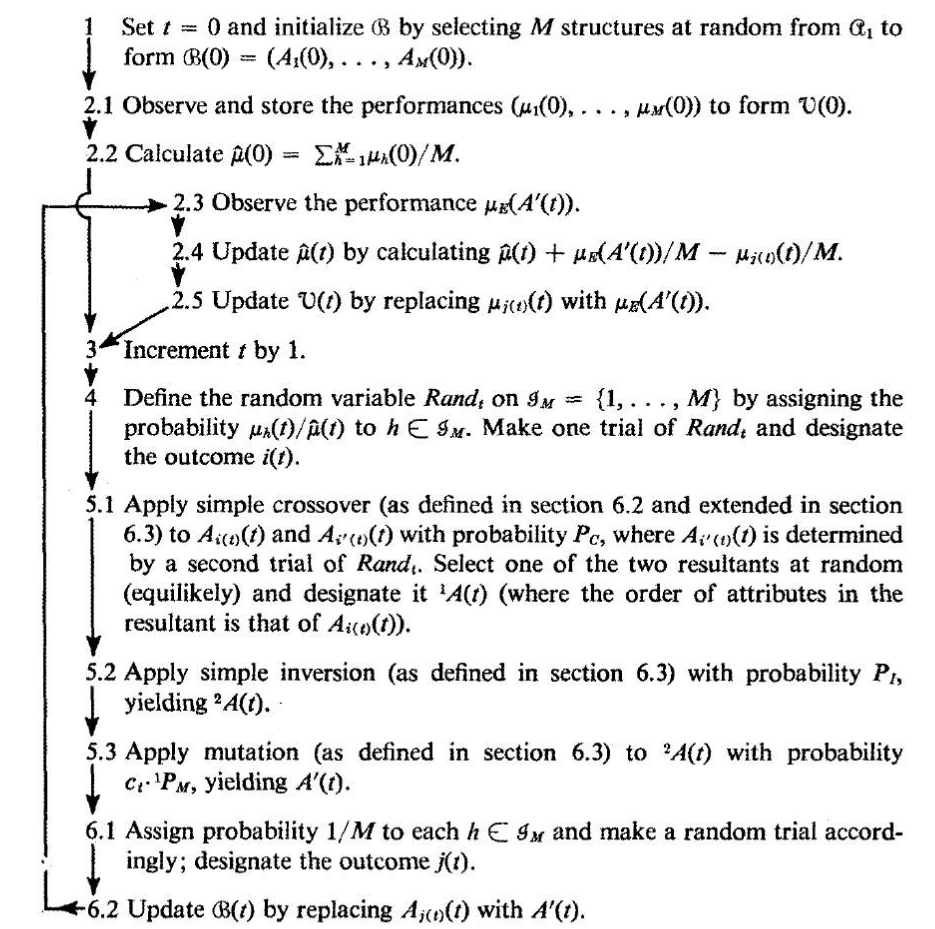
\includegraphics[width=\linewidth]{hollandAlg}
    \caption{GA outlined in Holland's Original Book\cite{hollandAdaptationNaturalArtificial1992}}
    \label{fig:hollandAlg}
\end{figure}

As you can see from Figure \ref{fig:hollandAlg} and Algorithm \ref{alg:GenericGA} the overall shape of GAs has not changed substantially over the course of the past 50 years. Being comprised of a series of operations that a starting population is piped through until criteria are met.

\subsection{Genetic Operators}\todo{Expand definitions of operators used in implementation section}
\label{subsec:GAOps}
In the following section I will outline the various genetic operations that take place in a GA, they can be seen in Algorithm~\ref{alg:GenericGA}. Any operators used and analysed in Chapter~\ref{chap:ClassicalApproach} will have more detailed explanations of their process.

\subsubsection{Selection}

The selection procedure is the process by which the next generation of individuals is created from the current population. Individuals are selected relative to their fitness as determined by the Objective (fitness) function $\mathcal{F}$. 

Some methods select only the best solutions by fitness. Others employ a more stochastic approach, such as roulette wheel selection, to increase diversity and reduce complexity.

\paragraph{Fitness-Proportional Selection}\label{imp:FitPropSel}

Fitness-proportional or Roulette wheel selection is a popular selection operator. It uses fitness to assign selection probability to each individual in a population.

The probability of selection for an individual $i$ with fitness $\mathcal{F}(i)$ can be expressed mathematically as:

\begin{equation}
    p_i = \frac{\mathcal{F}(i)}{ \sum^{N}_{j=1} \mathcal{F}(j)} 
\end{equation}

Where $N$ is the size of the population $P$

This is a simple approach but performs well and has very little performance overhead.

\paragraph{Ranked Selection}\label{imp:RankSel}

Ranked selection is an alternative selection method, it works on the assumption that the individuals in your population are closely grouped in fitness. The main difference of this method when compared to fitness-proportional selection is that it ranks individuals based on relative fitness rather than absolute fitness.

The procedure can be written mathematically as:

Given a population $P$ of size $n$ ordered by fitness. We select the top \(\gamma\)-ranked individual, $x_{\gamma}$ with a probability $p(\gamma)$. Where \(\gamma\) is the rank and $p(\gamma)$ is the ranking function.

The ranking function can take different forms including both linear and exponential ranking.\todo[inline]{extend list to include all functions used}

Linear ranking is defined as:

\begin{equation}
p(\gamma)= \frac{\alpha + (\beta-\alpha) \cdot \frac{\gamma}{n-1}}{n}
\end{equation}

Where:

\begin{itemize}
  \item $\sum_{\gamma=0}^n p(\gamma) = 1$
  \item $\alpha + \beta = 2$
  \item $1 \leq \beta \leq 2$
\end{itemize}

\subsubsection{Variation}

Variation in a GA is the process of altering the genome individuals to further explore the search space via stochastic local search.
We perform this using two distinct sub-operations: Mutation and Crossover.
Here we can view crossover as the \textit{breeding} process and mutation as resembling the natural tendency for DNA to mutate over the course of generations.

\paragraph{Mutation}
In mutation we alter each gene with a set probability $p_m$ known as the \textit{mutation rate}. A standard value for a mutation rate is $ \frac{1}{L} $ but it can fall anywhere in the range $p_m \in [ \frac{1}{L} , \frac{1}{2} ] $ where $L$ is the length of the genome.

A low value for $p_m$ a new individual which can be shown to be \textit{close} to it's parents in the search space relative to their \textit{Hamming distance}\footnote{Hamming Distance: A metric for comparing two binary data strings. The Hamming distance between two strings is the number of bit position in which they differ.} if using a Binary coded GA. In real-coded GAs they can be shown to be close by the Euclidean distance between them.

In binary coded GAs we alter a given gene by \textit{flipping} it's value.
In real-coded GAs mutation operators include: 
\begin{itemize}
    \item Uniform Mutation
    \item Non-Uniform Mutation
    \item Gaussian Mutation 
\end{itemize}
\subparagraph{Uniform Mutation}
In uniform mutation, we select a parent $p$ at random and replace a randomly selected gene $c_i \in p$ with a uniformly random number $c_i' \in [u_i,v_i]$  where $u_i$ and $v_i$ are set bounds.

\paragraph{Gaussian Mutation}

In Gaussian mutation, we select a parent $p$ at random and randomly select a gene $c_{i} \in p$. We replace $c_{i}$ with a new value $c_{i}'$ which is calculated as follows:

\begin{equation}
  c_{i}' = \min(\max(\mathcal{N}(c_{i},\sigma_{i}), u_{i}), v_{i})
\end{equation}

Where $\mathcal{N}(c_{i},\sigma_{i})$ is a Gaussian distribution with a standard deviation \(\sigma_{i}\) and a mean of $c_{i}$. \(\sigma_{i}\) may depend on the length of the interval bound, $l_{i} = v_{i} - u_{i}$, typically (and in my implementation) $\sigma_{i} = \frac{1}{10}l_{i}$


\subsubsection{Crossover}

Crossover is a binary operation, taking two randomly selected \textit{parents} from the population $P_t$ with a probability $p_c \in [0,1]$ 

There are two major forms of crossover for binary coded GAs: $n>1$ point crossover and Uniform crossover. 

For real-coded GAs you instead have a selection of Crossover operators including:

\begin{itemize}
    \item Flat crossover
    \item Simple crossover
    \item Whole arithmetic crossover
    \item Local arithmetic crossover
    \item Single arithmetic crossover
    \item BLX-$\alpha$ crossover
\end{itemize}


\subparagraph{Simple (one point) Crossover}\label{imp:SimpCross}

For simple crossover, randomly select a crossover point, $i \in \{1,\ldots,n \}$. All values before this point are swapped between the two parents. For 2 parents, $p_1 = \left\{ x_1^{[1]},\ldots,x_n^{[1]}\right\}$ and $p_2 = \left\{ x_1^{[2]},\ldots,x_n^{[2]}\right\}$ this can be represented as:

\begin{equation}
    p_1' = \left\{ x_1^{[1]},x_2^{[1]}, \ldots, x_i^{[1]}, x_{i+1}^{[2]},\ldots, x_n^{[2]} \right\} 
\end{equation}

\begin{equation}
    p_2' = \left\{ x_1^{[2]},x_2^{[2]}, \ldots, x_i^{[2]}, x_{i+1}^{[1]},\ldots, x_n^{[1]} \right\}
\end{equation}

\subsubsection{Evaluation}
After developing potential new individuals, the fitness of these new individuals is calculated using the objective function, $\mathcal{F}$

\subsubsection{Reproduction}
Here the next generation of individuals is constructed. There are multiple potential methods employed here with the simplest being to just replace the least fit individuals with additional copies of the fitter individuals, be they pre-existing or newly generated.

In this stage various heuristics or alternative strategies can be implemented to speed up or slow down the convergence rate. Whilst their fitness may be low, having a diverse population allows for more of the search space to be explored. If the algorithm converges too quickly it may get \textit{stuck} in local minima. 


\section{Bézier Curves}
\label{sec:back-bezier-curves}

In my implementation, I utilise Bézier curves to encode complex route arcs between a series of points. Here I will briefly outline their construction and mathematical basis.

Bézier curves were popularised by and named after French auto-body\footnote{so I feel it is quite fitting that they find use in $21^{st}$ century automotive problems} designer Pierre Bézier in the 1960s and are commonly found in computer graphics today. They are parametric curves made up of a series of \textit{control points} which contort the shape of a line to produce a curve of nearly any shape. Although their mathematical basis was established in 1912 by Sergei Bernstein in the form of Bernstein polynomials\cite{bernstein1912best}.

A Bézier curve is said to have a degree of $n-1$ where $n$ is the number of control points including the start and end point of the curve.

\subsection{Formal Definition}

Bézier curves can be simply and explicitly defined for degrees of 1 through 4, however, the general case of $n$ points is more useful to us. In their general form they can be defined recursively or explicitly. I implement the recursive version as it is much more readable for a programming language that supports recursion.

They are defined recursively as follows:

\begin{equation}
    \textbf{B}_{P_0}(t) = P_0
\end{equation}

\begin{equation}
    \textbf{B}_{P_0,P_1,\ldots,P_n}(t) = (1-t)\textbf{B}_{P_0,P_1,\ldots,P_{n-1}}(t) + t\textbf{B}_{P_1,P_2,\ldots,P_n}(t)
  \end{equation}

  Where the initial curve $B = B_{P_{0},P_{1},\ldots,P_{n}}$ and the parameter $t$ is a real number in the range of $[0,1]$. Therefore, the smoothness of the curve is determined by the granularity of the parameter when realising the curve.

An example of how the parameter $t$ corresponds to points on the curve can be seen in Figure~\ref{fig:bezexample}, the red numbers indicate the value for $t$ that corresponds to the green points on the curve and the purple points correspond to the control points. I.e. $B(0.37)$ produces the coordinates for the first labelled point seen, where the curve shown is $B$.

\begin{figure}[ht]
  \centering
  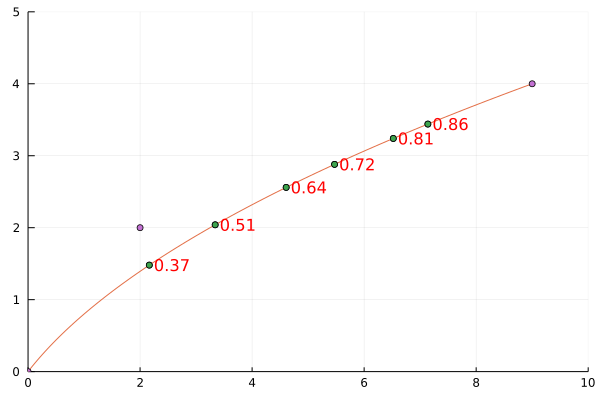
\includegraphics[scale=0.35]{figures/bezExample.png}
  \caption{\label{fig:bezexample} Example of a Bézier  curve with a random sample of points}
\end{figure}


\subsection{Length of a Bézier curve}
\label{subsec:back-bez-length}

The length of a Bézier curve is a non-trivial calculation and is best approximated as:

\begin{equation}
    L = \frac{(2L_c + (n-1)L_p)}{n+1}
\end{equation}

Where $L_c$ is chord length and $L_p$ is polygon length. This was proven by Jens Gravesen\cite{gravesenAdaptiveSubdivisionLength1997} in 1997.

Chord length is given by:

\begin{equation}\label{eq:bezlength}
  L_{c} = \sqrt{\left(P_{0_{x}} - P_{n_{x}}\right)^{2} + \left(P_{0_{y}} - P_{n_{y}}\right)^{2}}
\end{equation}
% √((first.x - last.x)^2 + (first.y - last.y)^2)

and polygon length by:

\begin{equation}
  L_{p} = \sum_{i=0}^{n-1} \sqrt{\left(P_{i_{x}} - P_{i+1_{x}}\right)^{2} + \left(P_{i_{y}} - P_{i+1_{y}}\right)^{2}}
\end{equation}

Or, alternatively:

\begin{equation}
  L_{p} = \sum_{i=0}^{n-1} L_{c}(B_{P_{i},P_{i+1}})
\end{equation}

\subsection{Subdivision of $n$-degree Bézier curves}
\label{sec:decasteljau}

Subdivision of Bézier curves is a key stage in the process of finding any intersections between two Bézier curves. The process of subdivision is performed using De Casteljau's algorithm. This algorithm was developed by Paul de Casteljau while working at Citroen in 1959 to work with the family of curves that would later be formalised into Bézier curves by Pierre Bézier\footnote{Bézier curves have also been called de Casteljau curves as much of his work preceded that of Pierre Bézier's}.

It is a simple procedure, given a Bézier curve $B$, it can be split at any arbitrary point $t \in [0,1]$ into two curves with control points of the form:

\begin{align}
  \beta_{1} &= B_{P_{0}}(t), B_{P_{0},P_1}(t), \ldots, B_{P_{0},\ldots,P_{n}}(t) \\
  \beta_{2} &= B_{P_{n}}(1-t), B_{P_{n},P_{n-1}}(1-t), \ldots, B_{P_{n},\ldots,P_{0}}(1-t)
\end{align}
\feedback{Should I change this superscript notation? subscript is being used to denote which control points are being considered.}

% \beta_1 = [ B[1:i](t) for i in 1:length(B) ]
% \beta_2 = [ B[i:length(B)](1-t) for i in length(B):-1:1 ]

\section{Fully Autonomous Road Networks}

Fully autonomous road networks are by no means a novel concept. They have appeared in fiction since the mid 20th century and have been a real possibility for the past decade. In a fully autonomous road networks \textit{(FARN)}s, all vehicles are self-operating with their routing either being determined on a vehicle-by-vehicle \textit{selfish} basis or by a larger system managing routes for all nearby agents. 

In the latter system protocols that promote the net increase in efficiency can be implemented. However, this sort of system will require a form of government mandate as a universal routing protocol would need to be established and implemented by all auto manufacturers; this is no small undertaking.

\section{Miscellaneous}

\subsection{Bounded Boxes}
\label{subsec:back_boundedboxes}

  A bounded box of a curve is defined as the box constructed from the points $(x_{min},y_{min}), (x_{min},y_{max}), (x_{max},y_{min}), (x_{max},y_{max})$ Where $x_{min,max}$ and $y_{min,max}$ are the minimum and maximum $x$ and $y$ values from all control points respectively. An example can be seen in Figure~\ref{fig:bboxeg}

 \begin{figure}[ht]
   \centering
   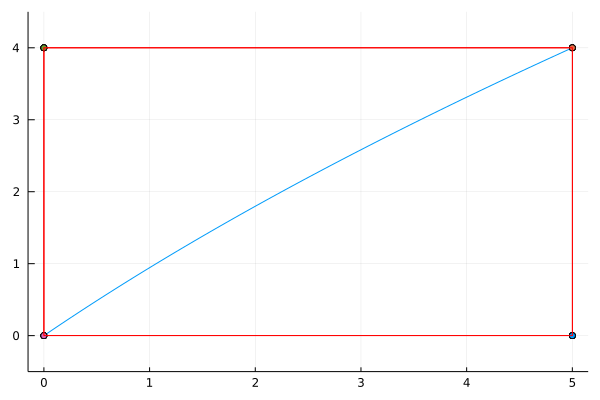
\includegraphics[scale=0.5]{figures/bbox_eg.png}
   \caption{\label{fig:bboxeg} A bounding box for a Bézier curve of degree 2}
 \end{figure}


%TC:macro \todo 1

%%% Local Variables:
%%% mode: latex
%%% TeX-master: "report"
%%% End:
